\documentclass[compass]{beamer}
\usepackage[latin1]{inputenc}
\usepackage[T1]{fontenc}
\usepackage{beamerthemesplit}
\usetheme{Warsaw}
\useoutertheme[subsection=false]{smoothbars}

\newtheorem{merkmale}{Merkmale}

\newtheorem{kasten}{}
\newtheorem{definiere}{Definition}

\title{Open Government, E-Government 2.0, Open Data}	

\author{Ulrich Viefhaus und Christian Lomp}

\institute{Seminar 1916 E-Government}

\logo{\pgfimage[width=1cm,height=1cm]{./images/logo.jpg}}

\date{1. Dezember 2010}

\begin{document}

\frame{\titlepage}

%!TEX root =  vortrag.tex
\section{Open Government}
\frame{
\frametitle{Open Government}

\begin{kasten}[Barack Obama "'Transparency and Open Government", 2009]
\begin{itemize}
 \item {\bf Government should be transparent} -- Transparenz f�rdert Rechenschaftspflicht und bietet Informationen f�r B�rger �ber das, was ihre Regierung tut.
 \item {\bf Government should be participatory} -- Partizipation verst�rkt�die�Effektivit�t�von�Regierung�und�Verwaltung�und�verbessert�die�  Qualit�t�ihrer�Entscheidungen.
 \item {\bf Government should be collaborative}  -- Kolaboration�bietet�innovative�Werkzeuge,�Methoden�und�Systeme, um�die�Zusammenarbeit�unter den Verwaltungen und mit der �ffentlichkeit zu st�rken.
\end{itemize}
\end{kasten}
}

\frame{
\frametitle{�ffnung von Staat und Verwaltung}

\begin{merkmale}[Open Government]
\begin{itemize}
  \item Transparenz
  \item Partizipation
  \item Kollaboration  
  \item Open Innovation  
  \item �ffnung gegen�ber der Gesellschaft
  \item Open Data
  \item Offene Standards, Offene Schnittstellen, Open Source
\end{itemize}
\end{merkmale}
}
\frame{
\frametitle{Transparenz}
\begin{merkmale}[Transparenz]
	\begin{itemize}
	\item Externe Nachvollziehbarkeit von Vorg�ngen und Entscheidungen in Politk, Verwaltung und Justiz.
	\item Umsetzung durch soziale Netzwerke, transparente Informationssysteme und offene,gemeinschaftliche Formen des Editierens� von�
Texten und Beitr�gen.
     \item �ffentlicher Zugang zu nicht-personenbezogenen und nicht geheimen Daten und Informationen der �ffentlichen Verwaltung (``'Open Data''').
\end{itemize}
\end{merkmale}
}

\frame{
\frametitle{Umfrage zur Transparenz}


\begin{figure}
\begin{center}
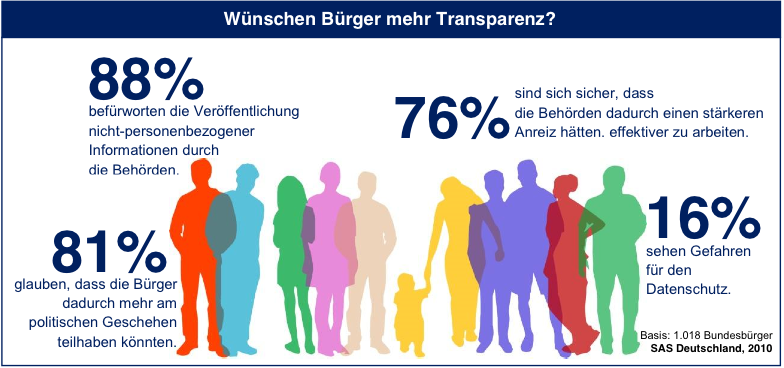
\includegraphics[width=10cm]{images/Transparenz_Umfrage.png}
\caption{Eine Forsa-Studie im Auftrag von SAS Deutschland, 2010	}
\end{center}
\end{figure}

}

%nicht-staatliche Beispiel Lobbypedia http://www.lobbypedia.de, Abgeordnetenwatch http://www.abgeordnetenwatch.de/

\frame{\frametitle{Partizipation}
	
\begin{merkmale}[Partizipation]
 \begin{itemize}
  \item Einbindung der B�rger in Entscheidungsprozessen von Politk und Verwaltung.
  \item Umsetzung durch offenen gemeinschaftlichen Dialog
  \item Meinungsbildung wird durch elektronische Medien Text, Bild, Ton und Video erg�nzt.
  \item ergebnisoffene B�rgerbefragungen
  \item Bewertungen und Meinungsbildgewinnung auf Knopfdruck
  \item moderierter Dialog, verteiltes Brainstorming
\end{itemize}
\end{merkmale}
}

\frame{\frametitle{Kollaboration}
 \begin{merkmale}[Kollaboration]
  \begin{itemize}
    \item Verst�rkte Einbindung von B�rgern, Unternehmen, Verb�nde und B�rgerinitiativen in die Aufgabenverteilung
zwischen Staat und Gesellschaft.
    \item Verst�rkte �bergreifende und interne Zusammenarbeit von Beh�rden (shared services)
    \item Einbindung von B�rgern, Verb�nden und Unternehmen in vorhandene Prozessketten.
    \item Schwarmauslagerung (``'Crowd Sourcing'''), z.B. durch Open Source, Government Mashups, AppStores, Hackdays
   \end{itemize}
 \end{merkmale}

}

\frame{\frametitle{Open Innovation}
 \begin{merkmale}[�ffnung des Innovationsprozesses]
  \begin{itemize}
    \item Innovation der Verwaltung durch Ideen der B�rger, Programmierer und Unternehmen.
    \item Protypen durch Datenportale oder Ideen-Wettbewerbe (``'Apps4Government''')
    \item Innovationsprozess als Wirtschaftsf�rderungsma�nahme.
    \item Personalpolitik
   \end{itemize}
 \end{merkmale}
}


\frame{
\frametitle{�ffnung gegen�ber der Gesellschaft}
 \begin{merkmale}[�ffnung gegen�ber der Gesellschaft]
  \begin{itemize}
    \item Ziele: aktiver Austausch und ergebnisoffener Dioalog und Diskurs von B�rgern und Verwaltung
    \item Ausrichtung der Verwaltung auf Bed�rfnisse und Probleme der B�rger f�hrt zu erh�hter B�rgerzufriedenheit
    \item partnerschaftliches Verh�ltnis, gegenseitiges Vertrauen.
   \end{itemize}
 \end{merkmale}
}

\frame{
 \frametitle{Open Data}
 \begin{merkmale}[Open Data]
  \begin{itemize}
  \item Beh�rdendaten und mit �ffentlichen Mitteln finanzierte Daten �ffentlich zug�nglich machen.
  \item Vollst�ndige  Prim�rquellen, zeitnah nach ihrer Generierung.
  \item Keine Diskriminierungen und  Einschr�nkungen beim Zugriff.
  \item Vernetzung der Daten
  \item Generiern neuen Wissens (``'HackDays''')
  \item Freie unlizensierte Inhalte wie Texte, Bild-,Ton- und Filmwerke (z.B. Dt. Digitale Bibiothek oder Digt. Bildarchiv des BAarch)
   \end{itemize}
 \end{merkmale}
}

\frame{
 \frametitle{Offene Standards, Offene Schnittstellen}
 \begin{merkmale}
  \begin{itemize}
  \item Grundlage f�r offene Kommunikationssysteme  
  \item Interoperabilit�t durch Offenheit, z.B. Datenformat ODF
  \item Europ�ischer Interoperabilit�tsrahmenwerk 
  \end{itemize}
 \end{merkmale}
}

\section{E-Government 2.0}
\frame{\frametitle{Web 2.0 Technologie}
\begin{itemize}
\item Blogs,� Wikis� und� offene� Redaktionssysteme� erm�glichen� ein gemeinsames,�verteiltes Editieren von Texten.�
\item Foren und Beratungsdienste�er�ffnen�Formen�des�gemeinschaftlichen�Diskutierens. 
\item Gemeinschaftlichen�Entscheidungsfindung�und� verteiltes� Programmieren.
\item Transparente, partizipative und kollaborative Ans�tze� zur Verwaltungsmodernisierung durch Web 2.0 
\end{itemize}
}


\frame{
\frametitle{Blogs -- Weblog,�Mikroblog,�Fotoblog,�Podcast, Webcast�}
{\footnotesize
\begin{kasten}[Einsatzfelder]
(Mikro-)Blog�von�Politikern/Beh�rden, Fotoblog von Veranstaltungen, Podcasts
\end{kasten}
\begin{kasten}[Nutzen, St�rken, Chancen]
Direkte,�authentische�Information, erweitertes Info-Angebot, Newsfeed, kommentieren ohne technisches Know-How, ungefilterte pers�nliche Sichten
\end{kasten}
\begin{kasten}[Schw�chen und Risiken]
Zeitaufwand, Motivation, fehlende Qualit�tssicherung
\end{kasten}
}
\begin{center}
\includegraphics{images/facebook}

\includegraphics{images/twitter}

\includegraphics{images/youtube}

\includegraphics{images/flickr}

\includegraphics{images/blogger}

\includegraphics{images/rss}\end{center}
%
\includegraphics[width=10cm]{SozialeNetze.png}
}

\frame{
\frametitle{Beispiele Podcast, Twitter, Facebook}
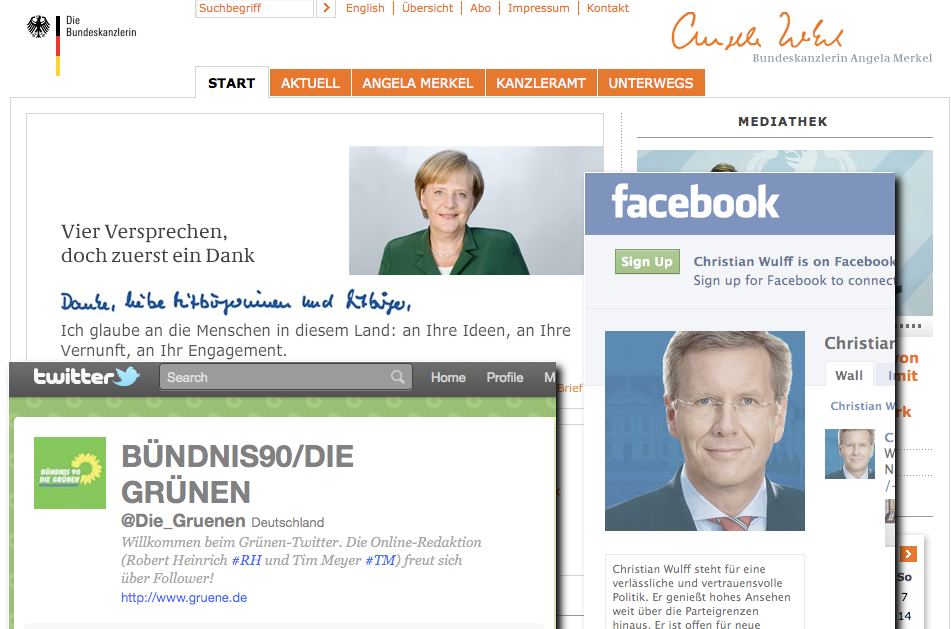
\includegraphics[width=0.9\textwidth]{images/Merkel}
}


{\usebackgroundtemplate{
\includegraphics[transparent]{images/wikipedia}}
\frame{
\frametitle{Wikipedia}
{\footnotesize
\begin{kasten}[Einsatzfelder]
Au�endarstellung �ber Lexikabeitr�ge
\end{kasten}

\begin{kasten}[Nutzen, St�rken, Chancen]
Interaktives Beteiligungsformat; Hochwertige Form der Aufbereitung von Beitr�gen;
Aktive Gestaltung durch die Bev�lkerung; Offenheit, Transparenz, Aktualit�t; weltweit abrufbar.
\end{kasten}

\begin{kasten}[Schw�chen und Risiken]
Qualit�t und Korrektheit der Inhalte variiert (Autorenexpertise, Manipulationen und falsche Eintr�ge)
\end{kasten}}
}
}

\frame{
\frametitle{Hamburg Stadtwiki}
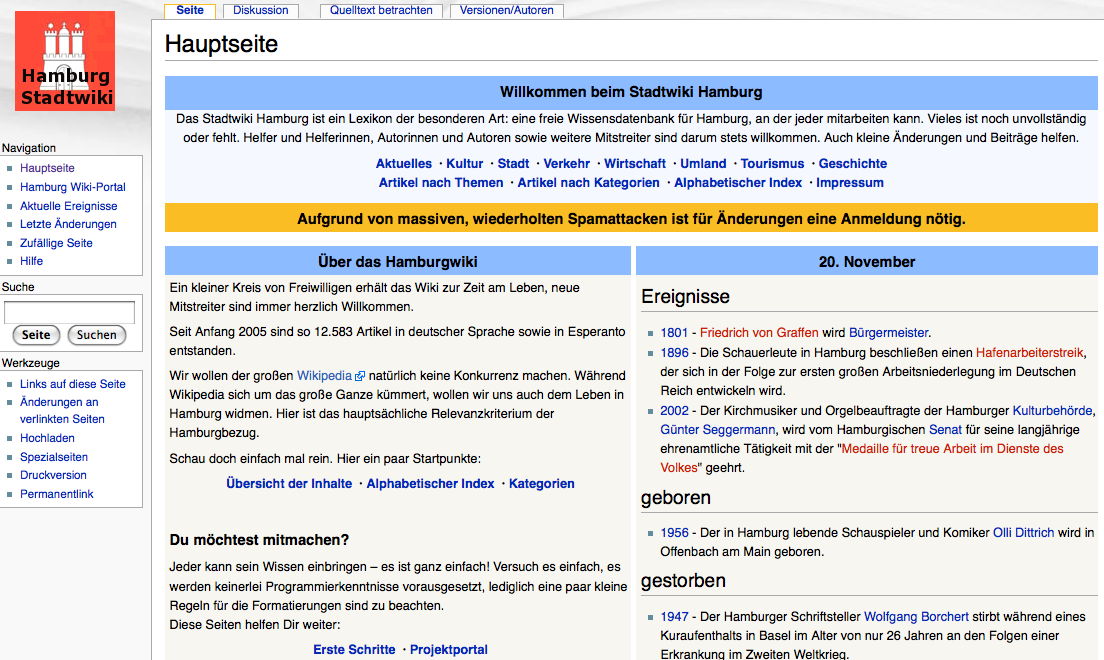
\includegraphics[width=0.9\textwidth]{images/Stadtwiki}
}
\frame{
\frametitle{Stadt- und Regiowiki}
{\footnotesize
\begin{kasten}[Einsatzfelder]
Interaktives�Beteiligungsformat durch frei zug�ngliche�Stadt?oder�Regiowikis.
\end{kasten}

\begin{kasten}[Nutzen, St�rken, Chancen]
Interaktives Beteiligungsformat; Private�Verwertung, Bearbeitungen�und Weitergabe der�Inhalte�zul�ssig;
breites�Informationsangebot;�� 
\end{kasten}

\begin{kasten}[Schw�chen und Risiken]
Verwertung�ohne�finanzielle�R�ckfl�sse�an die�Autoren; Urheberrechte�und�Rechtsverst��e; Qualit�t und Korrektheit der Inhalte variiert (Autorenexpertise, Manipulationen und falsche Eintr�ge)�� 
\end{kasten}}
}



\frame{
\frametitle{B�rgerhaushalt: K�ln}
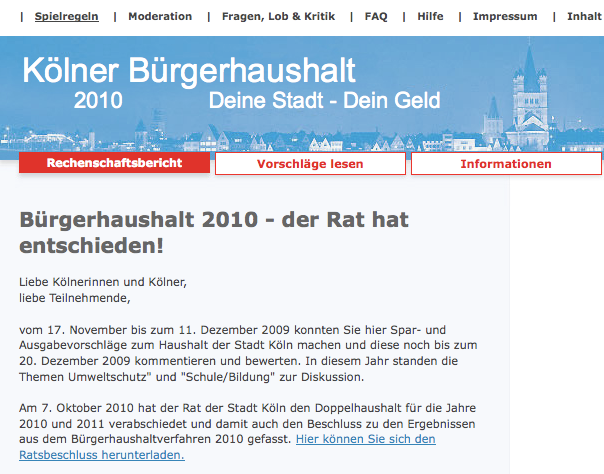
\includegraphics[width=0.9\textwidth]{images/Buergerhaushalt}
}

\frame{
\frametitle{B�rgerhaushalte}
{\footnotesize\begin{kasten}[Einsatzfelder]
Information�und�Kommunikation�``Wohin�gehen�unsere�Steuergelder?''; Offene�Einreichung und Bewertung�von�Vorschl�gen� 
\end{kasten}

\begin{kasten}[Nutzen und St�rken]� 
Beitrag�zur�Verwaltungsmodernisierung; Entwicklung�von�Probleml�sungen durch Verwaltung und B�rger;
H�here�Akzeptanz�der�Haushaltsentscheidung; Einbindung/Mitverantwortung der�B�rger�als�Impulsgeber/Betroffene; Vermeidung�einer�digitalen�Spaltung durch�einen�vertikalen�Mehrkanalansatz�� 
\end{kasten}

\begin{kasten}[Schw�chen]
Qualifizierungsbedarf�der�B�rger und Verwaltungsmitarbeiter;
Zus�tzlicher�Aufwand/Kosten eines B�rgerhaushalts; Dominanz�Einzelner;
Entmachtung�der�gew�hlten�Vertreter; Desinteresse
\end{kasten}
}}


\frame{
\frametitle{Dashboard: Offener Haushalt}
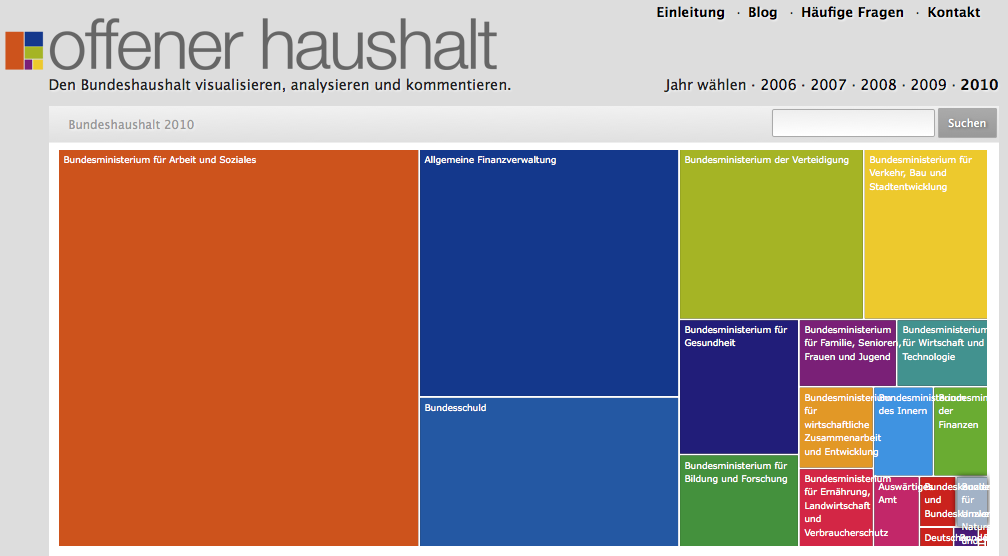
\includegraphics[width=\textwidth]{images/OffenerHaushalt}
}


\frame{
\frametitle{Dashboards}
{\footnotesize\begin{kasten}[Einsatzfelder]
�bersicht��ber�laufende Projekte/Haushalt
\end{kasten}
\begin{kasten}[Nutzen und St�rken]� 
Ad?hoc?Auskunft�in Echtzeit; Vereinfachtes,�verst�ndliches�Berichtswesen (Informationsfluss);
Erh�hung�der�Transparenz; Visualisierung�von�komplexen�Informationsmengen; Interesse;  Beitrag�zur�Korruptionsbek�mpfung�� 
\end{kasten}

\begin{kasten}[Schw�chen]
Aufbereitung�der�Rohdaten�erforderlich (Zeit/Kosten);
Hohe�Transparenz�zeigt�Schw�chen�des�Systems (Presse)
\end{kasten}
}}
\frame{
\frametitle{IT-Dashboard}
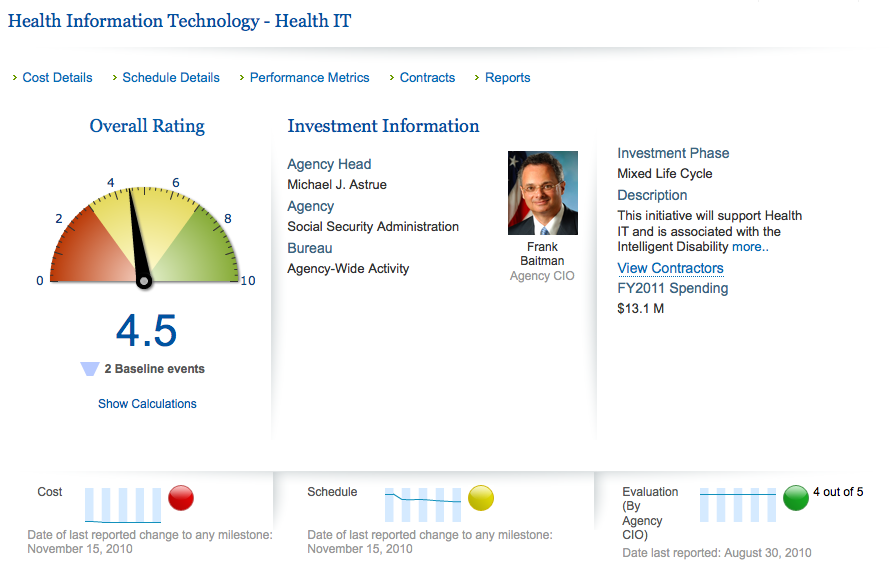
\includegraphics[width=\textwidth]{images/Dashboard}
}



\frame{
\frametitle{Offene Datenportale}
{\footnotesize\begin{kasten}[Einsatzfelder]
Datenportale�zu�freien�Verwaltungsdaten; Apps�for�Democracy?Wettbewerbe� 
\end{kasten}
\begin{kasten}[Nutzen und St�rken]
Vereinfachter und freier�Zugang�zu�Rohdatenbest�nden; Daten�als�Basis�f�r�qualifizierte�Entscheidungen, demokratische�Prozesse und Forschung; Innovationstreiber,�Wirtschaftf�rderung
\end{kasten}
\begin{kasten}[Schw�chen]
Kosten des�Datenkatalogs;�Urheberrechte;  Auswahl�der�Datenbest�nde; 
``Vermischung''��ffentlicher�und�privater Dienstleistungen
\end{kasten}
}}

\frame{
\frametitle{Offene Datenportale}
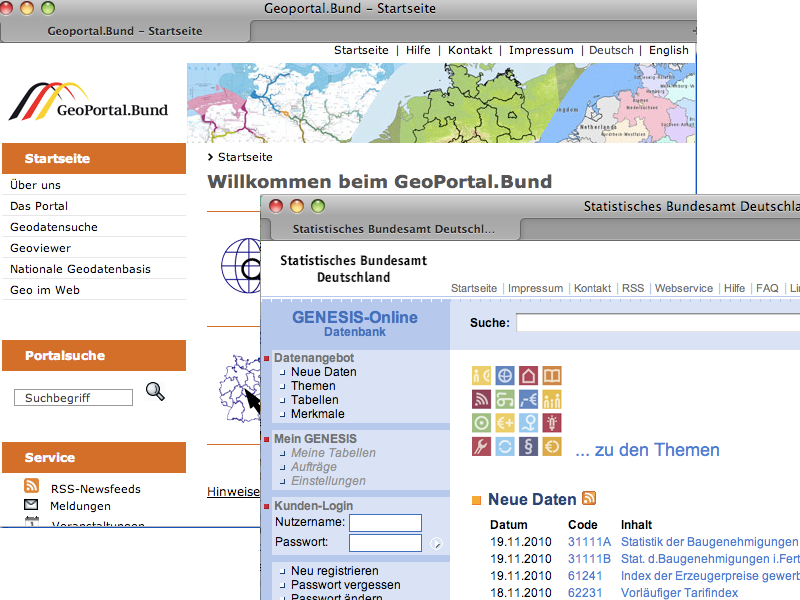
\includegraphics[width=0.9\textwidth]{images/Datenportale}
}

\frame{
\frametitle{Gov Camps and Hack Days}
{
\footnotesize 
\begin{kasten}[Einsatzfelder]
BarCamps�f�r�Web�2.0-Interessenten; HackDays�f�r�Programmierer� 
\end{kasten}
�
\begin{kasten}[Nutzen und St�rken]
Vernetzung�der�Akteure; Austausch von vielf�ltigen Ideen und �ber neue Werkzeuge; Vielfalt�der�Themen�und hochwertige�Vortr�ge; Gewinnung�neuer�Partner�und�F�rderer.
\end{kasten}

\begin{kasten}[Schw�chen]� 
Bloߠgrobe�inhaltliche�Vorplanungen�m�glich; fehlende Qualit�tssicherheit;
Selbstorganisation�und Eigendynamik
\end{kasten}

\includegraphics[width=4cm]{images/GovCamp}
}}



\section{Open Data}
\frame{
\frametitle{Open Data}

\begin{merkmale}
Mekrmale von OpenData
\end{merkmale}}


\end{document}
